\section{Design of the method}

\begin{figure}[htb!]
\centerline{
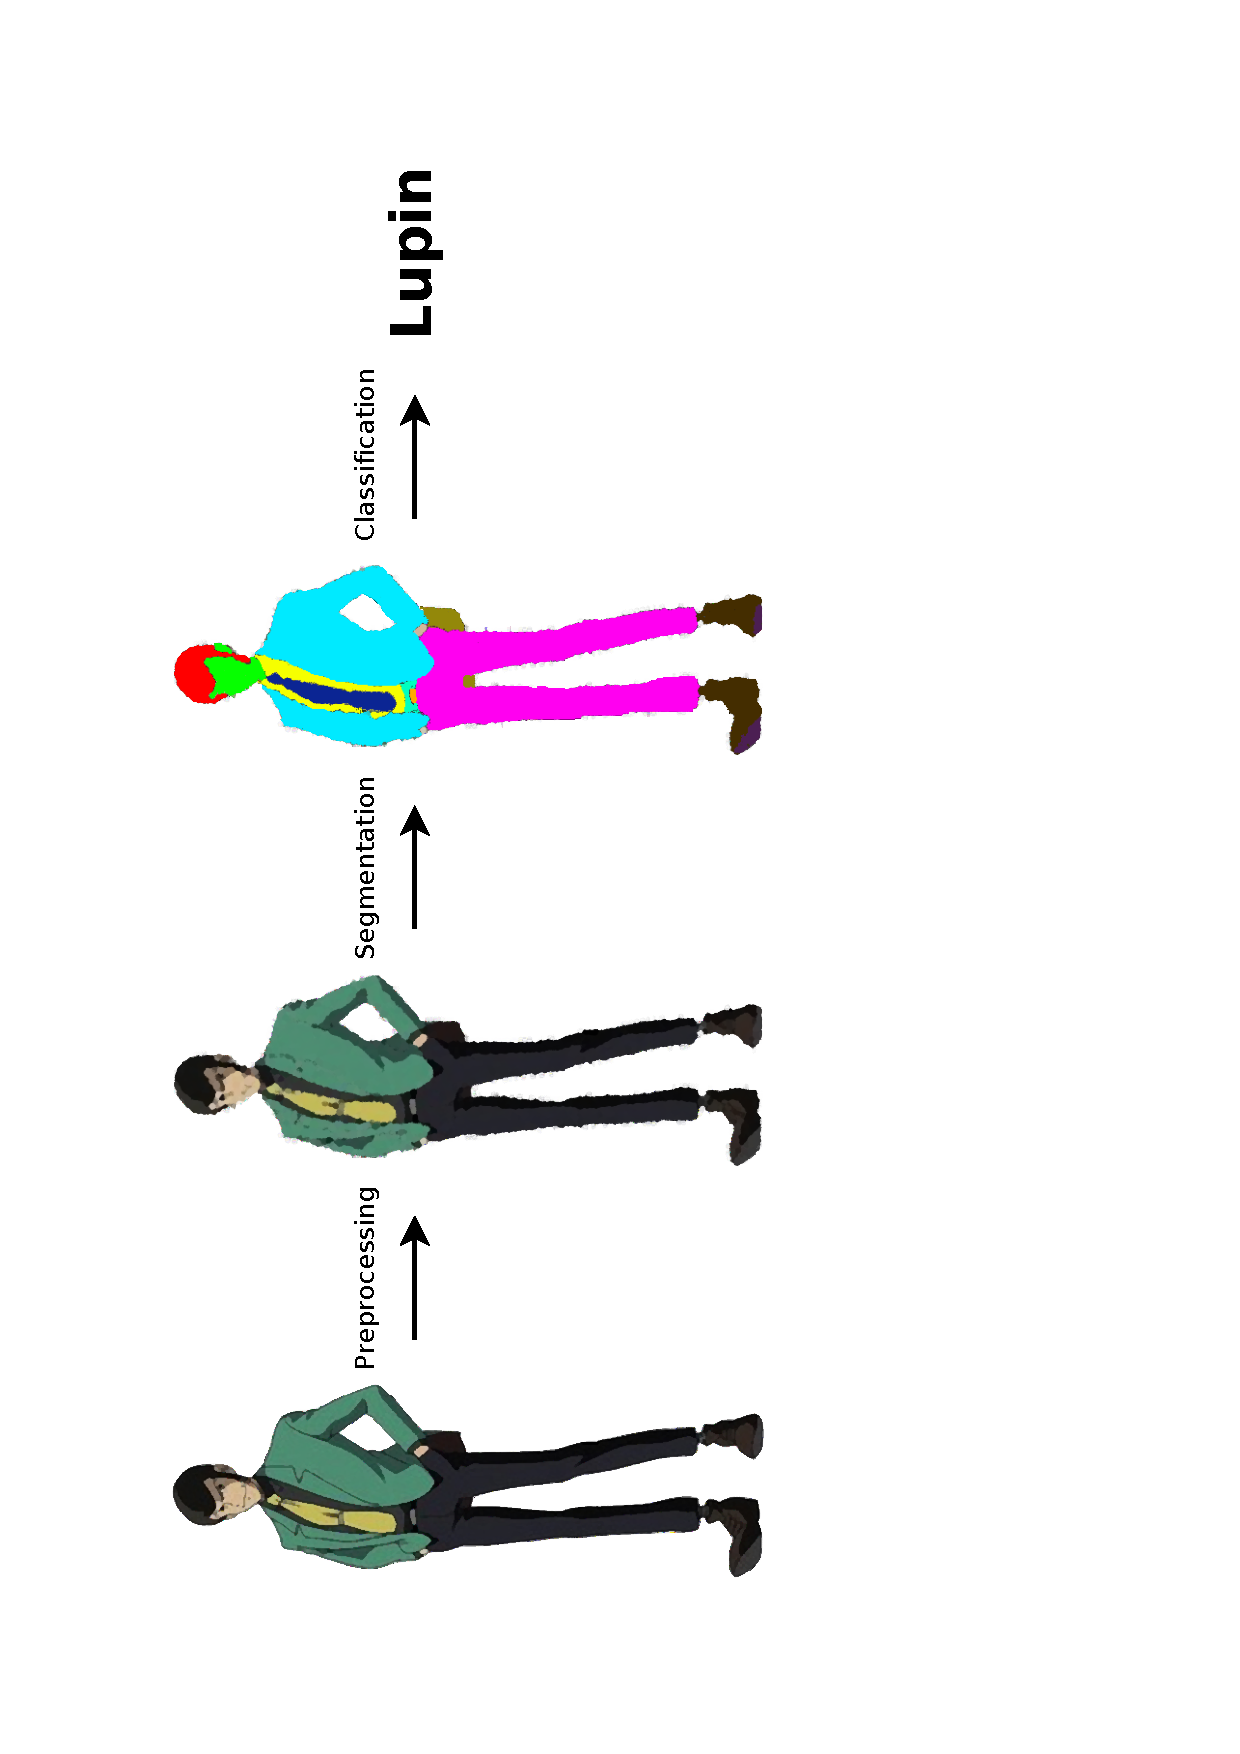
\includegraphics[height=1.2\textwidth,angle=270,clip=true,trim=0 0 6cm 0]{images/visionSystemDiagram.pdf}
}
\caption{Diagram depicting how preprocessing, segmentation and classification interact.}
\end{figure}

The method takes the shape of computer vision system with separate phases of preprocessing, segmentation and classification.

\begin{itemize}
\item The preprocessing step should operate transformations on the original image so segmentation can be applied efficiently and accurately. This includes filtering, color space transformations, histogram manipulations and geometric transformations. This results into a new preprocessed image.
\item The segmentation method aims to automatically isolate parts of the character image as faithfully to human perception as possible. An ideal segmentation would for instance segment separately hair, face, clothes, hands and feet as separate components.
The end result of the segmentation is a partition of the set of pixels in the image.
\item The goal of classification is to extract features of interest from the segmentation, and use these features to predict the character identity from the training information. The end result is the predicted name of the character.
\end{itemize}

Although the global structure of the method described above did not change during design, many techniques were experimented with for each of the steps. In this section each technique will be described. See \autoref{sec:conventions} in the appendices for the mathematical conventions and definitions used in this document, which although not departing from standard rely heavily on vocabulary from spectral graph theory, image processing and fuzzy logic.

\subsection{Preprocessing}
\subsubsection{Kuwahara filter}
\begin{figure}[htb!]
\centering
\begin{subfigure}{.24\textwidth}

\includegraphics[width=\textwidth]{images/miku_d.png}
\caption{Before filtering.}
\end{subfigure}
\begin{subfigure}{.24\textwidth}

\includegraphics[width=\textwidth]{images/miku_d_filtered_smallh.png}
\caption{Small window.}
\end{subfigure}
\begin{subfigure}{.24\textwidth}

\includegraphics[width=\textwidth]{images/miku_d_filtered.png}
\caption{"good" window.}
\end{subfigure}
\begin{subfigure}{.24\textwidth}
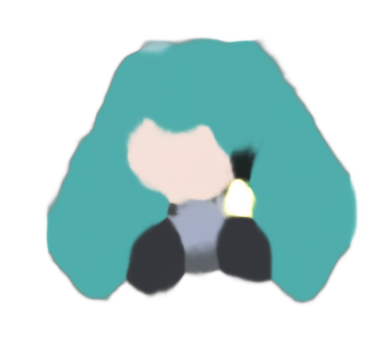
\includegraphics[width=\textwidth]{images/miku_d_filtered_largeh.png}
\caption{Large window.}
\end{subfigure}
\caption{Results of Kuwahara filtering with varying window size. The small window causes outlines to be accentuated, and the large window removed the tie, ribbon and legs.}
\label{fig:kuwaharaExample}
\end{figure}

One of the early issues encountered when attempting to segment animation character images was the presence of black outlines, which usually get segmented into many large components, but do not contain any information relevant to identification. We identified the Kuwahara filter \cite{kuwahara1976processing} as a way to not only remove the black outlines, but also remove other unnecessary details and make area of color more homogeneous and amenable to segmentation.

\paragraph{The method} Consider a grayscale image $I$ (we'll see later how it generalizes to color images). For each point $(x,y)$ on $I$, we consider a square window of size $2h + 1$ centered on it. We then consider $4$ overlapping square regions in this window as shown in \autoref{fig:kuwaharaQuadrants}. For each such region $Q_i$ for $i \in \{1, ..., 4\}$ we compute the arithmetic mean $m_i(x,y)$ and standard deviation $\sigma_i(x,y)$ of pixel values inside $Q_i$. The pixel value at $(x,y)$ in filtered image $J$ is then defined as the arithmetic mean $m_i(x,y)$ corresponding to the smallest standard deviation $\sigma_i(x,y) = \min_{j \in \{1, ..., 4\}}\sigma_j(x,y)$. When dealing with borders of the image, we simply do not consider the missing pixels while computing the means and variances.

\begin{figure}[htb!]
\centering
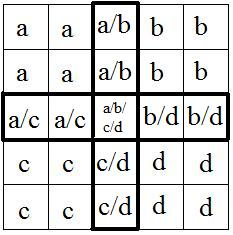
\includegraphics[width=0.3\textwidth]{images/kuwahara_quadrants.jpg}
\caption{Window used by the Kuwahara filter with half-size $h = 2$ and square regions $a$, $b$, $c$ and $d$.}
\label{fig:kuwaharaQuadrants}
\end{figure}

Generalizing to color images, we still consider the arithmetic means of pixel colors, but this time we consider the brightness of the pixels (e.g. the V in HSV color space) for standard deviation.

\paragraph{Theoretical justification} The algorithm was originally designed to improve segmentation in medical image processing. For the case of removing outlines, if one considers a window size "large enough" that outlines never fills most of it, then it will introduce a large standard deviation in the square region it is contained in - meaning it will be removed in the filtered image. It should be noted that if the window is not large enough, then outlines can actually be thickened by the Kuwahara filter, and if it is too large then relevant information may be lost (\autoref{fig:kuwaharaExample}). We found however that it is easy do empirically determine a window size in practice.

\paragraph{Implementation} A naive implementation of the filter recomputes all means and variances for each pixel, runs in $O(nh^2)$ time where $n$ is the number of pixels in the image, and $h$ is the window half size.

\subsubsection{Color space selection}

As the goal is to obtain a segmentation as close to human perception as possible, the $L^*a^*b^*$ color space has been found to be most suitable. The $HSV$ or $HSL$ color spaces are also useful to extract hue information, (the $H$ in either color space) which we use for histogram equalization (\autoref{sec:histEq}) and as post-processing to segmentation (\autoref{sec:hueMerging}).

Although using $L^*a^*b^*$ color space gives good segmentations, it may not be ideal for classification as $2$ different characters may share predominantly the same color palette. A possible extension of this would be to use training data to determine an abstract and possibly non-linear color space where members of the same class are close and members of different classes are far away, using - for instance - a (semi) supervised embedding method similar to the one used in \cite{urahama2007semi}.

\subsubsection{Color histogram equalization by hue}
\label{sec:histEq}

Some characters are represented predominantly by a few colors, which makes segmentation more difficult. Equalizing the histogram by hue allows segmentation to distinguish between more closely related colors, and therefore distinguish some colors which would be otherwise close in color space. The drawback beinng that irrelevant differences in color space are also accentuated, so histogram equalization was eventually removed from preprocessing as it had an overall negative impact on segmentation performance.

\subsection{Segmentation}
\subsubsection{Felzenszwalb's method}
The segmentation method by P. F. Felzenszwalb and D. P. Huttenlocher, described in detail in \cite{felzenszwalb2004efficient}, is an efficient graph-based segmentation method for color images.

\paragraph{The method} Let $I$ be a color image. The algorithm considers a graph $G = (V,E)$ defined on the set of pixels of I with weight function $w$ measuring dissimilarity between pixels. Let $n$ be the number of vertices and $m$ the number of edges of $G$. The pseudo code of the algorithm is given in \autoref{alg:felzenszwalb}, where $MInt : S \times S \rightarrow \mathbb{R}^+$ for some segmentation $S$ is defined by:
\[
MInt(C_1, C_2) = \min(Int(C_1) + \tau(C_1), Int(C_2) + \tau(C_2))
\]
$\tau(C) = \frac{k}{|C|}$ is a threshold function for a scale parameter $k$, and $Int(C)$ measure the internal difference of a component $C$, defined by
the largest weight of the minimum spanning tree of $C$:
\[
Int(C) = \max_{\{u,v\} \in MST(C, E)} w(u,v)
\]

\begin{algorithm}
\caption{Felzenszwalb's segmentation algorithm}
\label{alg:felzenszwalb}

\begin{algorithmic}[1]
\Function{Felzenszwalb}{$G = (V, E)$}
\State Sort $E$ into $\pi = (o_1, ..., o_m)$ by ascending edge weights
\State Initialize $S_0$ with each vertex in its own component
\For{$q \gets 1$ to $m$}
\State Let $\{u,v\} = o_q$ the $q^{th}$ edge in the ordering
\State Let $C_u$ and $C_v$ the components containing $u$ and $v$ in $S_{q-1}$
\If{$C_u \neq C_v$ and $w(u,v) \leq MInt(C_u, C_v)$}
\State $S_q$ is obtained by merging $C_u$ and $C_v$ in $S_{q-1}$
\Else
\State $S_q$ is just $S_{q-1}$
\EndIf
\EndFor
\Return $S_m$
\EndFunction
\end{algorithmic}
\end{algorithm}


\paragraph{Theoretical justification} The authors show that this algorithm results in a segmentation which is neither too coarse nor too fine, according to a precise notion of boundary between segments. This is interesting for animation character images, which are characterized by large areas of homogeneous color, which this algorithm capture reasonably well.

\paragraph{Implementation} The algorithm can be implemented to run very efficiently. Using a disjoint set forest data structure for the segmentation allows the $Find$ and $Union$ operation to be performed in amortized $O(\alpha(n))$ time where $\alpha$ is the inverse of the Ackermann function, and computing $MInt$ between each iteration can be done in constant $O(1)$ time. With an adjacency list data structure for the graph $G$, it is easy to list all edges in $O(m)$ time. This makes clear that the time behavior of the algorithm is dominated by the initial sorting of edges, which can be computed in $O(mlog(m))$ time using an optimal comparison sort like merge sort.

The authors study the case where $G$ is an $8$-connected graph and where it is a variation on the $K$-nearest-neighbor graph\footnotemark
\footnotetext{
While a non-mutual $K$-nearest neighbor graph is not necessarily sparse, the authors assert that it is in their paper. As their graph construction is also not made explicit in the paper, and their source code only include an $8$-connected graph, we proceed under the optimistic assumption that the authors use a variation on the $K$-nearest-neighbor graph which is actually sparse.
}
 in $(x, y, r, g, b)$ feature space. Since both classes of graphs are sparse - the number of edges is within a constant factor of the number of vertices - this makes the time complexity of the algorithm $O(nlog(n))$.


\paragraph{Results and analysis} Although this algorithm is efficient, it suffers from a few drawbacks. The method as described above tends to create many very small components, which can be solved by a post-processing step greedily merging components smaller than a threshold. It also tends to produce segments of similar size, which in the case of animation character image is not desirable. It produces either an oversegmentation where large segments are separated in many small ones, or an undersegmentation where smaller segments are incorrectly merged into larger ones.

\begin{figure}[htb!]
% TODO: figure showing segmentation results for varying k
\caption{Segmentation results with Felzenszwalb's method, with a small $k$ and a larger $k$.}
\label{fig:felzenszwalbSegmentationResults}
\end{figure}

\subsubsection{Spectral segmentation and clustering algorithms}

\subsubsection{Felzenszwalb's method with hue-based segment merging}


\subsection{Classification}
\subsubsection{Tree-walk kernel}
Our initial idea for classifying the animation characters is to consider the region adjacency graph on the segments of the image. The intuition is that although changes in posture, scale change the overall image significantly, the arrangement of segments in the image relative to each other should roughly stay the same. Classifying images by their region adjacency graph has been studied by Z. Harchaoui and F. Bach in \cite{harchaoui2007image}, in which they a introduce a number of kernels to compute similarity between such graphs. We chose to study and implement the tree-walk kernel presented in this paper.

\paragraph{The method} Let $I$ be a color image, $S = \{S_1, ..., S_q\}$ a segmentation of $I$ and a $4$-connected notion of adjacency between pixels. The region adjacency graph $G$ of $I$ is defined as the graph where vertices are segments and there is an edge between segments $S_i$ and $S_j$ if and only if there is a pair of adjacent pixels $(p_i, p_j) \in S_i \times S_j$. As the $4$-connected graphs are always planar, and the region adjacency graph is a minor of the $4$-connected graph, the region adjacency graph is planar by Wagner's theorem. It should be noted however that the $8$-connected graphs are not planar beyond a grid of size 5 by 5 vertices by Euler's formula on planar graphs, and so using an $8$-connected notion of adjacency could be inappropriate for this method.

Let $G$ and $H$ be region adjacency graphs with labeling functions $l_g : V(G) \rightarrow L$ and $l_h : V(H) \rightarrow L$, where $L$ is a segment label set. The method considers a kernel function $k : L \times L \rightarrow \mathbb{R}^+ \cup \{0\}$ which measures similarity between segment labels. The authors first define the $p$-th order walk kernel $k_{\mathcal{W}}^p(G,H)$ between $G$ and $H$ as:

\[
k_{\mathcal{W}}^p(G,H) = \sum_{\substack{(r_1, ...., r_p) \in \mathcal{W}_G^p\\ (s_1, ...., s_p) \in \mathcal{W}_G^p}} \prod_{i=1}^p k(l_G(r_i), l_H(s_i))
\]

where $\mathcal{W}_G^p$ (resp $\mathcal{W}_H^p$) denotes the set of walks of length at most $p$ in $G$ (resp $H$).

\subsubsection{Segmentation graph spectral classification methods}
The tree walk kernels method performed poorly in part because it relies overly on the region adjacency graph of the image, whose structure changes significantly with image variations. In an effort to match graph structure more loosely, we considered the results from spectral graph theory which attempt to analyze graphs through the eigenvalues and eigenvectors of its Laplacian. Works by Wilson, Zhu, Hancock and Luo showed that such spectral methods could be used for graph pattern matching, including image classification through shock graphs \cite{wilson2005pattern}\cite{wilson2008study}. Furthermore, works in graph cut algorithms and application to clustering \cite{ng2002spectral} and segmentation\cite{shi2000normalized}\cite{meila2001random} showed that the eigenvectors of the Laplacian corresponding to smaller eigenvalue encode in a sense the global structure of the graph, while ignoring smaller details. We hoped this would allow the method to be robust to variations in animation character images.

\paragraph{The method} For each segmentation $S$, we consider $m$ features $(f_i : S \Rightarrow \mathbb{R}_i^q)_{1 \leq i \leq m}$. For instance, we used average $L*a*b*$ color, gravity center and area of the segment as features. For each feature $f_i$, we compute the $K$-nearest neighbor graph $G_i$ on $S$ with edges weighted by the Gaussian kernel $w(S_u,S_v) = e^{-\frac{||f_i(S_u) - f_i(S_v)||^2}{\sigma_i^2}}$, and its corresponding combinatorial Laplacian  $L_i$ (see \autoref{sec:laplacians} for definitions).




\subsubsection{Segment matching method}


\section{Possible improvements and extensions}
\label{sec:extensions}
\subsection{Using training data to determine an ideal color space}

The segment matching method, although it performs best in practice compared to the other methods, has trouble distinguishing characters drawing from a similar color palette.

Right now, the method uses the $L^*a^*b^*$ color space to compare colors against each other during prediction. The rationale behind this choice is that the $L^*a^*b^*$ color system aims to be perceptually uniform, and therefore is close in some sense to human perception. However, this may not be a desirable feature for classification, as different characters may share perceptually similar color palettes. 

Using this reasoning, we could use training data to derive an "abstract" color space for ideal clustering of the training data. In such a color space, humanly imperceptible nuances of color between characters could be significant, while perceptually large differences between samples for the same character could be smoothed out.

Let us consider a color image $I$, and its color histogram $H_I$ with $k$ bins per channels. If we take the average color of each of the $l$ most represented bins, we get some sort of color palette for the image. If we consider $n$ labelled (or possibly unlabelled) training images in $c$ classes, we can consider these colors as our new training samples labelled with the label of the original image. Embedding this data in some higher-dimensional space where it would be linearly separable - using manifold learning methods with a kernel function taking into account training data such as the one in \cite{urahama2007semi} for instance - could give us a color subspace on which to project new test samples before classification.

It is however unclear how one would avoid the curse of dimensionality in this case - we would need a $cl$-dimensional space to make sure each color of each character is linearly separable. As the segment matching method only relies on euclid distance in feature space, one could easily apply the kernel trick to the algorithm to tackle the issue. How such a kernel would incorporate training information remains to be solved, however. Further study of the literature on manifold learning, including methods for dimensionality reduction \cite{roweis2000nonlinear}
\cite{belkin2003laplacian}
\cite{saul2006spectral}, spectral clustering \cite{shi2000normalized}
\cite{grady2006isoperimetric}
\cite{ng2002spectral}
\cite{meila2001random} and semi-supervised classification \cite{urahama2007semi} could provide an answer to these questions.

\subsection{Further study of segmentation graph based methods}
\label{sec:extensionSegGraph}
A straightforward generalization of the segment matching method would have consider not just one-to-one relations on the sets of segments, but $k$-to-$k$ for small $k$. Enumerating all such possible combinations may however be intractable. Drawing inspiration from the tree walk kernels method \cite{harchaoui2007image}, one could use a graph structure on the set of segment to reduce the size of the space to explore - for instance a $K$-nearest neighbor graph. This leads us to consider sequences of distinct, adjacent segments on this graph, e.g. paths on length $k$ on the graph. Using reasoning similar to the ones in \cite{harchaoui2007image}, one might be able to derive efficient dynamic programming implementations to compute similarities between all such paths - as all $3$ features we consider can be computed efficiently for sets of segments from the features of the individual segments.

Such a generalization would make the hue-based segment merging step of segmentation, which is mostly heuristic and greedy, mostly redundant using a proper graph structure. Further, although such graphs have proven insufficient on their own for animation image classification, perhaps this graph structure on the images can be beneficial to distinguishing characters with otherwise similar features.

This reasoning also makes clear that the segment matching method is related in some sense to the tree walk kernels method. Although our method lacks a sound theoretical grounding, the tree walk kernel doesn't and studying how they relate might provide important information about our method. Namely, and as has been mentioned in the previous section, our algorithm could easily benefit from the kernel trick.

\subsection{Background extraction}
Right now, our method expects animation character images whose background has already been removed - manually in the case of our dataset. In practice however, and as can be easily seen in web artist communities, animation images typically have a background, which rarely ever contains information relevant to identification. Background extraction or removal would therefore be a necessary step for our method to be useful in practice.

In the case of human images, the state of the art to identify the human when there is background present is to detect the face of the person using a method such as the Viola-Jones algorithm \cite{viola2004robust}, and then to use a state of the art face recognition method such as the Eigenfaces or Fisherfaces algorithm \cite{turk1991eigenfaces} \cite{belhumeur1997eigenfaces}.

This technique cannot be directly applied to animation characters, as the face information is almost never relevant to identification - there is both too much variations by drawing style and too much uniformity in the way animation character faces are drawn for this. We would like to consider ideally the full body of the character, or at least a large part of the body.

We could still apply the Viola-Jones algorithm to detect the important parts of the character for identification - for instance hair, face, clothes, arms and legs - by using proper training data. Using some kind of abstract skeleton describing how these parts should be structured in the image, perhaps for different types of postures, one could then reasonably extract the entire body from the background. Our segment matching algorithm - or an improvement over it - can then identify the character.

There are however still many hurdles on the way to solve this problem, and many experiments to perform to test our hypothesises.